\documentclass{article}

% if you need to pass options to natbib, use, e.g.:
%     \PassOptionsToPackage{numbers, compress}{natbib}
% before loading neurips_2021

% ready for submission
\usepackage[final]{neurips_2021}

% to compile a preprint version, e.g., for submission to arXiv, add add the
% [preprint] option:
%     \usepackage[preprint]{neurips_2021}

% to compile a camera-ready version, add the [final] option, e.g.:
%     \usepackage[final]{neurips_2021}

% to avoid loading the natbib package, add option nonatbib:
%    \usepackage[nonatbib]{neurips_2021}

\usepackage[utf8]{inputenc} % allow utf-8 input
\usepackage[T1]{fontenc}    % use 8-bit T1 fonts
\usepackage{hyperref}       % hyperlinks
\usepackage{url}            % simple URL typesetting
\usepackage{booktabs}       % professional-quality tables
\usepackage{amsfonts}       % blackboard math symbols
\usepackage{nicefrac}       % compact symbols for 1/2, etc.
\usepackage{microtype}      % microtypography
\usepackage{xcolor}         % colors
\usepackage{amsmath}
\usepackage{verbatim}
\usepackage[mathscr]{euscript}
\usepackage{graphicx}
\title{Machine Learning, 2024 Spring\\Assignment 7}
% The \author macro works with any number of authors. There are two commands
% used to separate the names and addresses of multiple authors: \And and \AND.
%
% Using \And between authors leaves it to LaTeX to determine where to break the
% lines. Using \AND forces a line break at that point. So, if LaTeX puts 3 of 4
% authors names on the first line, and the last on the second line, try using
% \AND instead of \And before the third author name.



\begin{document}

\author{
    Name: \textbf{Zhou Shouchen} \\\\
	Student ID: 2021533042
}

\maketitle

\begin{abstract}

\end{abstract}
\newpage

\textcolor{blue}{Problem 1}
Referring to Figure 4.10, why are both curves increasing with $K$? Why do they converge to each other with increasing $K$? (20pt)
\begin{figure}[htbp]
    \centering
    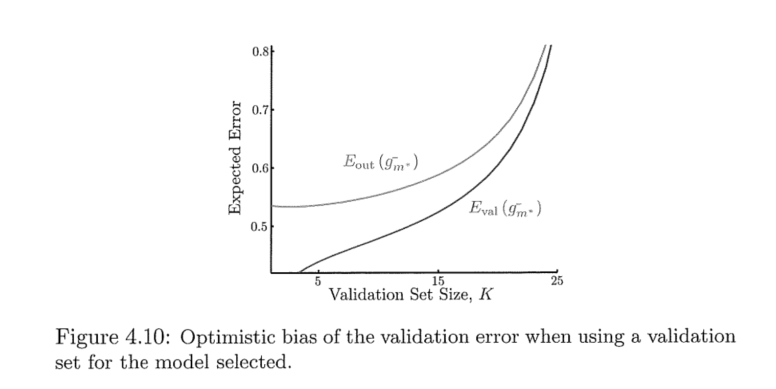
\includegraphics[width=1.0\textwidth]{../fig/figure.png}
\end{figure}
\par 
\textcolor{blue}{Solution}











\newpage
\textcolor{blue}{Problem 2}
\begin{enumerate}
    \item From Figure 4.12, $\mathbb{E}[E_{out}(g^-_{m^*})]$ is initially decreasing. How can this be, if $\mathbb{E}[E_{out}(g^-_{m^*})]$ is increasing in $K$ for each $m$? (10pt)
    \item From Figure 4.12 we see that $\mathbb{E}[E_{out}(g_{m^*})]$ is initially decreasing, and then it starts to increase. What are the possible reasons for this? (10pt)
    \item When $K=1$, $\mathbb{E}[E_{out}(g^-_{m^*})]<\mathbb{E}[E_{out}(g_{m^*})]$. How can this be, if the learning curves for both models are decreasing? (10pt)
\end{enumerate}
\begin{figure}[htbp]
    \centering
    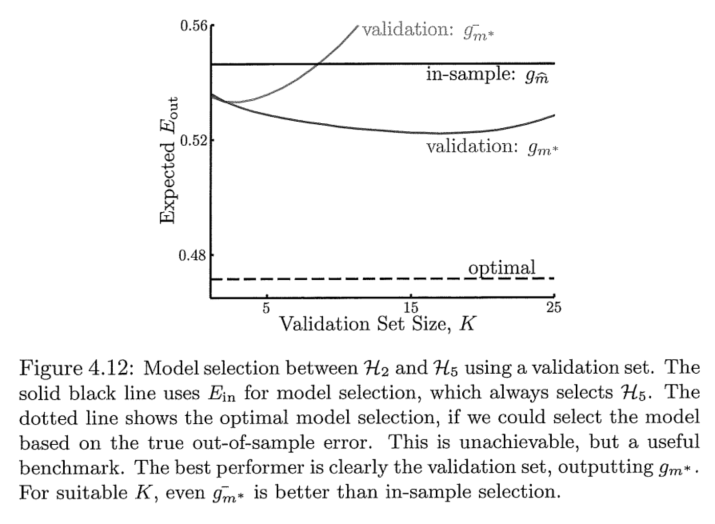
\includegraphics[width=0.8\textwidth]{../fig/figure412.png}
\end{figure}
\par


\textcolor{blue}{Solution}\\
1.\\
(a) Initally, the size of validation set $K$ is quite small, so it would not be able to provide a good estimate of the generalization error. As $K$ increases, the estimate of the generalization error becomes more accurate, so $\mathbb{E}[E_{out}(g^-_{m^*})]$ initially decreases.\\
(b) Similarly to te Problem 1, the size of the total data is fixed, so as $K$ is large enough, then as $K$ increases, there are less points used for training. We can assume that are data points are useful data, so less data points used for training will lead to a worse model. And it is reasonable that the performence of the model both on training set and validation set will decrease. i.e. $\mathbb{E}[E_{out}(g^-_{m^*})]$ increases.

So above all, as $K$ increases, the $\mathbb{E}[E_{out}(g^-_{m^*})]$ is initially decreasing, when $K$ is large enough, $\mathbb{E}[E_{out}(g^-_{m^*})]$ is increasing in $K$ for each $m$ as $K$ increases.

2. The understanding of the notions:\\
The models are $\mathcal{H}_1,\cdots,\mathcal{H}_M$, we first train with training data $\mathcal{D}_{\text{train}}$ to train all models, and use the cross-validation to get the best model $\mathcal{H}_{m^*}$, with error $g^-_{m^*}$ on the validation set $\mathcal{D}_{\text{val}}$. Then the total dataset $\mathcal{D}$ is used for training the model $\mathcal{H}_{m^*}$, and the error on the test set $\mathcal{D}_{\text{test}}$ is $g_{m^*}$.\\
So with the understanding of notions, we can get that:\\
$\mathbb{E}[E_{out}(g_{m^*})]$ is only relevant to the model we selected. When $K$ is small, as $K$ increases, $\mathcal{D}$ is quite close to $\mathcal{D}_{\text{train}}$, so it is similar to $g^-_{m^*}$, so $\mathbb{E}[E_{out}(g_{m^*})]$ decrease as we can choose the good model with cross validation.\\
When $K$ is large enough, as $K$ increases, less useful data are in $\mathcal{D}_{\text{train}}$, although we can choose a good trained model among $\mathcal{H}_1,\cdots,\mathcal{H}_M$, but the best trained model is not good enough, so the error $\mathbb{E}[E_{out}(g_{m^*})]$ on the test set $\mathcal{D}_{\text{test}}$ is increasing.\\

So above all, $\mathbb{E}[E_{out}(g_{m^*})]$ decreases initially, and then it increases as $K$ increases.\\

3. A possible reason is that $K=1$ is too small that even though the models are well trained, the $g_{m^*}$ could have a small $E_{\text{in}}$, but could not make sure that $E_{\text{out}}$ is small.\\
But $g^-_{m^*}$ is trained with cross-validation, so it is more likely to have a good $E_{\text{out}}$ as it is selecting the best model on $\mathcal{D}_{\text{val}}$.
So we have when $K=1$,
$$\mathbb{E}[E_{out}(g^-_{m^*})]<\mathbb{E}[E_{out}(g_{m^*})]$$

\newpage
\textcolor{blue}{Problem 3}
\par \textbf{Definition 1 (leave-one-out cross-validation)} \textit{Select each training example in turn as the single example to be held-out, train the classifier on the basis of all the remaining training examples, test the resulting classifier on the held-out example, and count the errors.}
\par Let the superscript -i denote the parameters we would obtain by finding the SVM classifier $f$ without the $i$th training example. Define the \textit{leave-one-out CV error} as
\begin{equation}
    \frac{1}{n}\sum_{i=1}^n\mathcal{L}(y_i,f(\mathbf{x}_i;\mathbf{w}^{-i},b^{-i})),
\end{equation}
where $\mathcal{L}$ is the zero-one loss. Prove that
\begin{equation}
    \text{leave-one-out CV error}\leq \frac{\text{number of support vectors}}{\text{n}}
\end{equation} (20pt) \\
\textcolor{blue}{Solution}

















\newpage
\textcolor{blue}{Problem 4}
\par The $l_1$-norm SVM can be formulated as follows
    \begin{equation}
       \begin{aligned}
        \min_{\mathbf{w},b} & \|\mathbf{w}\|_1 \\
        \text{s.t. }& y_i(\mathbf{w}^T\mathbf{x}_i+b)\leq 1,i=1,...,n.
    \end{aligned}     
    \end{equation}

\par Please deprive the equivalent linear programming formulation of (3) (10pt), give its dual formulation (10pt). Also, please explain how to determine the support vector SV according to the optimal multiplier. (10pt) \\
\textcolor{blue}{Solution}

















\end{document}